\subsection{Api}
	La componente \textit{Api} permette all'applicazione web di interfacciarsi con due differenti database: un database relazionale (PostgrSql) al cui interno sono contenute ad esempio le informazioni riguardanti gli utenti, gli enti e le configurazioni dei gateway, mentre nel database timeseries (Timescale) sono contenuti i dati dei sensori ricevuti dai gateway.
	Infine tramite le api, la web-app può interfacciarsi con un bot Telegram ed inviare vari tipi di notifiche;
	\subsubsection{Diagramma dei package}
		Data la numerosità delle classi all'interno della componente Api del progetto ThiReMa si è deciso di inserire il diagramma dei package per chiarificare le relazioni tra le classi che verranno poi illustrate in seguito.
		\begin{figure}[H]
			\centering
			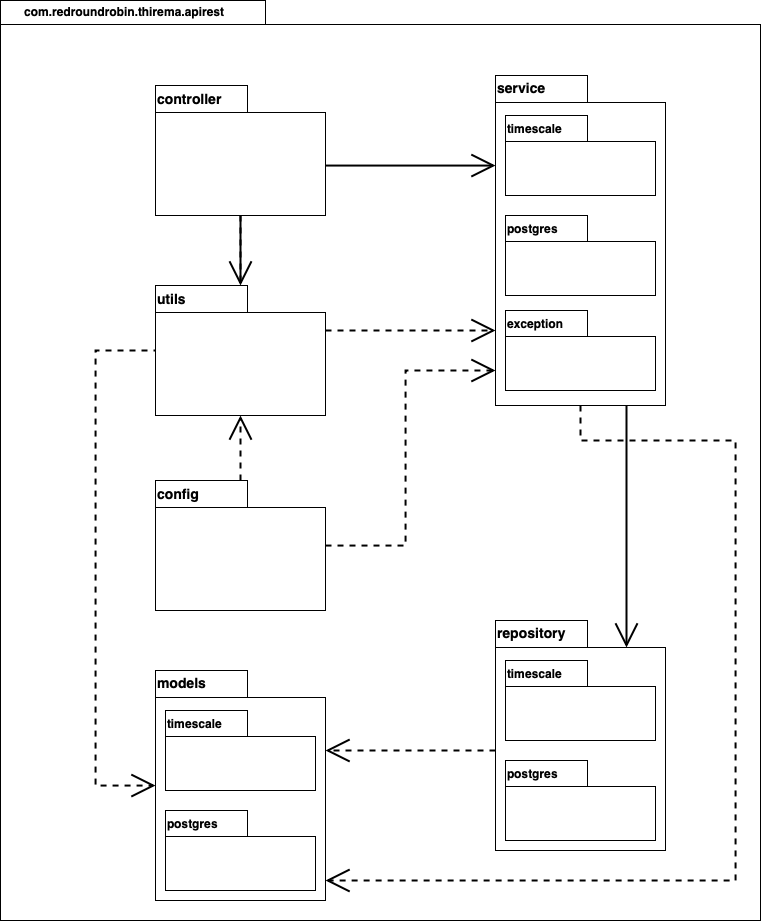
\includegraphics[scale=0.600]{res/images/API/packageAPI.png}
			\caption{Diagramma dei packages per la componente Api}
		\end{figure}

	\subsubsection{Diagrammi delle classi}
		Al fine di semplificare la comprensione delle dipendenze della componente Api, si è deciso di suddividere i diagrammi per package, mostrando solo quelli più significativi.

		%No models b0ss
		\begin{figure}[H]
			\centering
			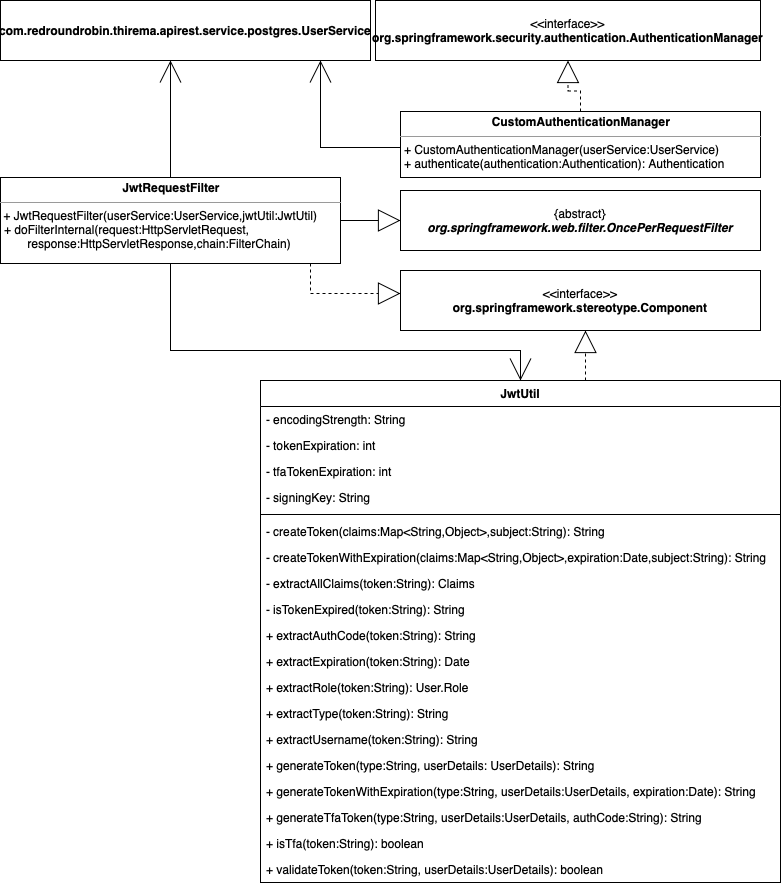
\includegraphics[scale=0.500]{res/images/API/UtilsPackage.png}
			\caption{Diagramma del package Utils della componente Api}
		\end{figure}
		\begin{figure}[H]
			\centering
			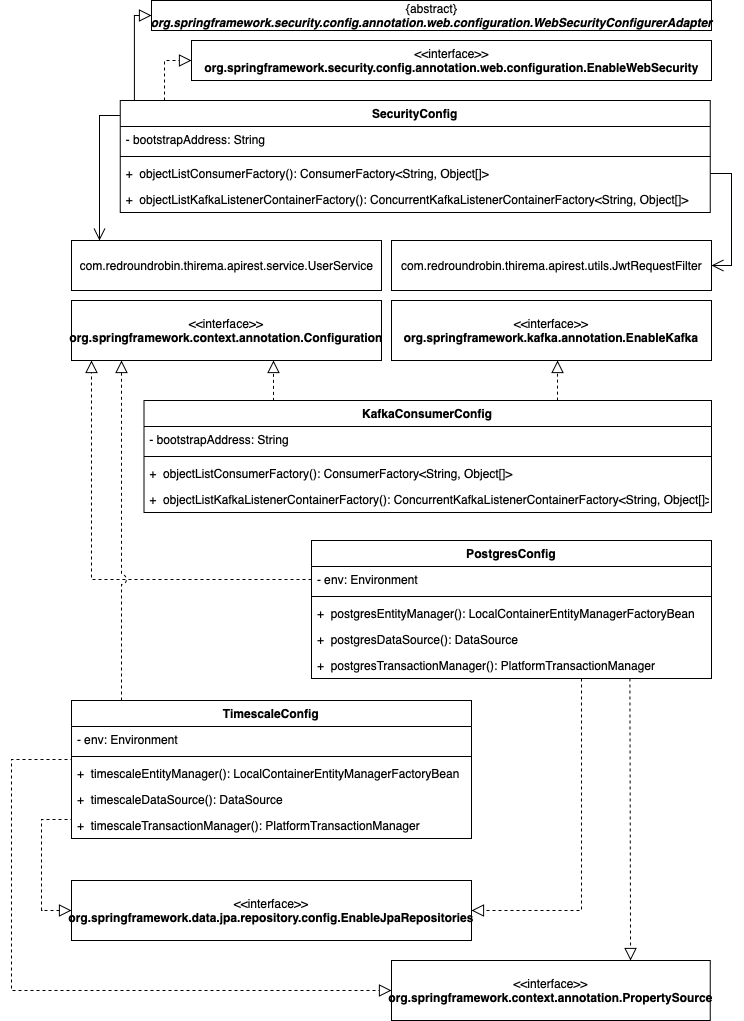
\includegraphics[scale=0.550]{res/images/API/ConfigPackage.png}
			\caption{Diagramma del package Config della componente Api}
		\end{figure}
		\begin{landscape}
		\begin{figure}[H]
			\centering
			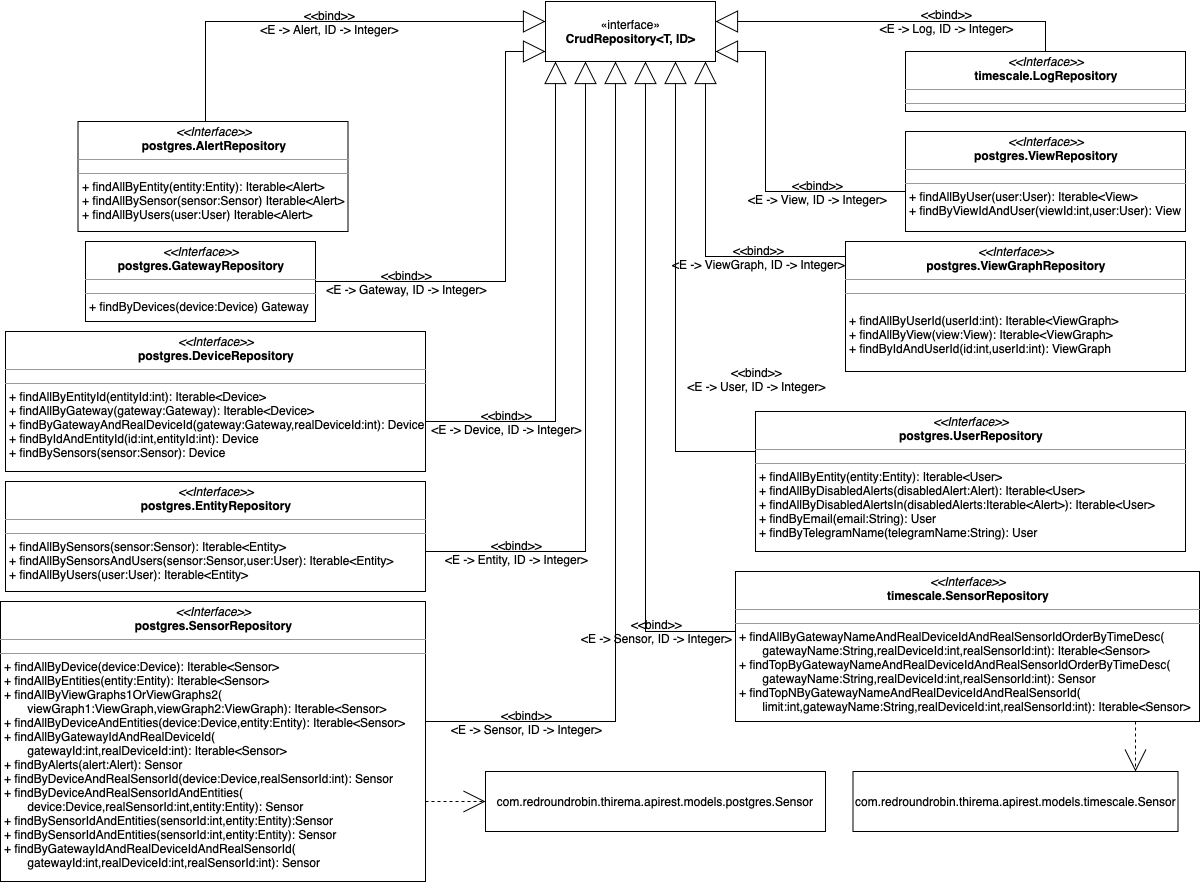
\includegraphics[scale=0.550]{res/images/API/RepositoryPackage.png}
			\caption{Diagramma del package Repository della componente Api}
		\end{figure}
		\begin{figure}[H]
			\centering
			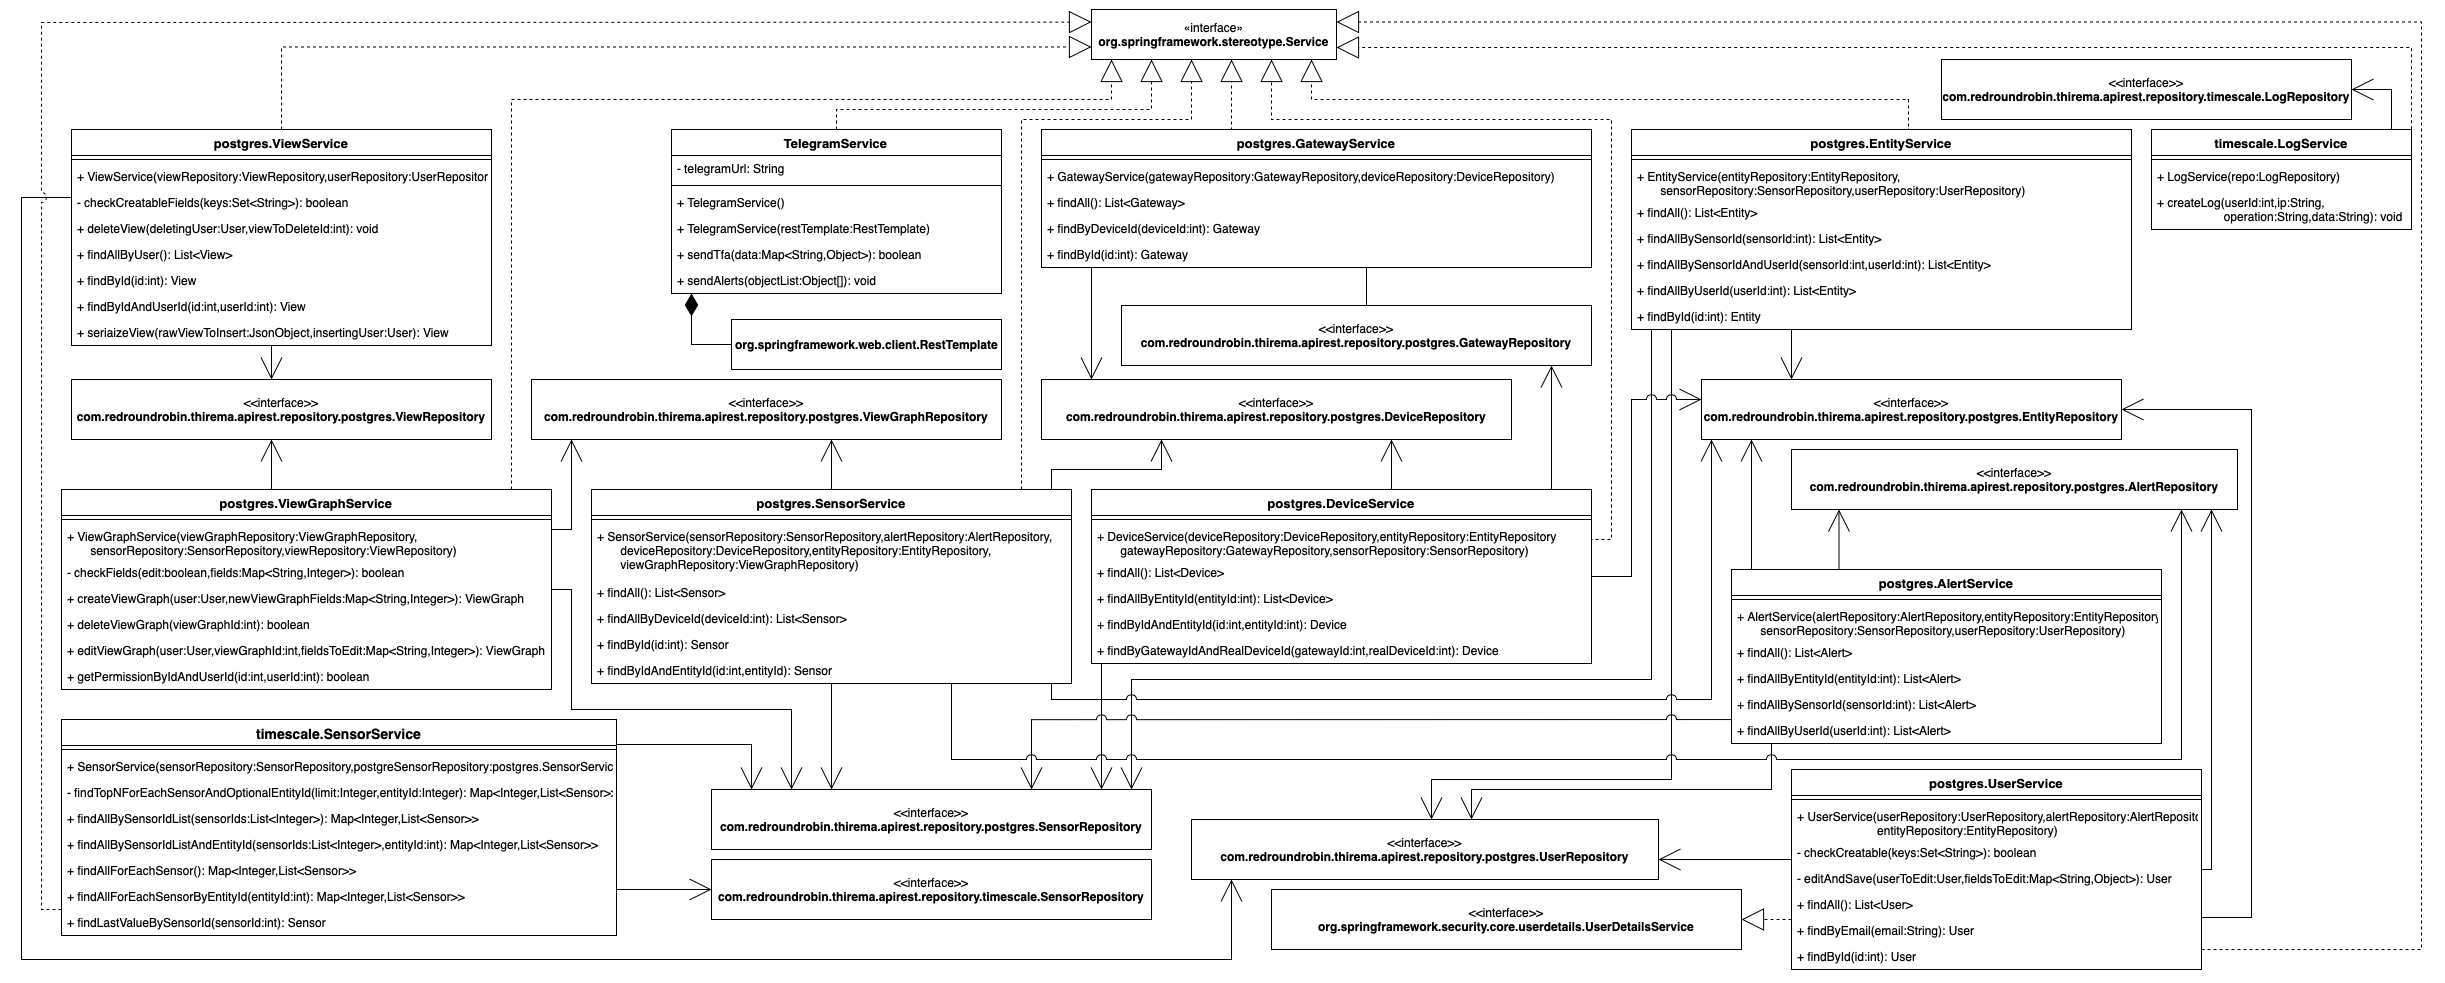
\includegraphics[scale=0.300]{res/images/API/ServicePackage.png}
			\caption{Diagramma del package Service della componente Api}
		\end{figure}
		\end{landscape}
		%%%%%%%%%%%%%%%%%%%%%%%%%%%%%Manca controllers%%%%%%%%%%%%%%%%%%%%%%


